\documentclass[14pt]{extbook}
\usepackage{multicol, enumerate, enumitem, hyperref, color, soul, setspace, parskip, fancyhdr} %General Packages
\usepackage{amssymb, amsthm, amsmath, latexsym, units, mathtools} %Math Packages
\everymath{\displaystyle} %All math in Display Style
% Packages with additional options
\usepackage[headsep=0.5cm,headheight=12pt, left=1 in,right= 1 in,top= 1 in,bottom= 1 in]{geometry}
\usepackage[usenames,dvipsnames]{xcolor}
\usepackage{dashrule}  % Package to use the command below to create lines between items
\newcommand{\litem}[1]{\item#1\hspace*{-1cm}\rule{\textwidth}{0.4pt}}
\pagestyle{fancy}
\lhead{Makeup Progress Quiz 2}
\chead{}
\rhead{Version B}
\lfoot{2790-1423}
\cfoot{}
\rfoot{Summer C 2021}
\begin{document}

\begin{enumerate}
\litem{
Which of the following equations \textit{could} be of the graph presented below?
\begin{center}
    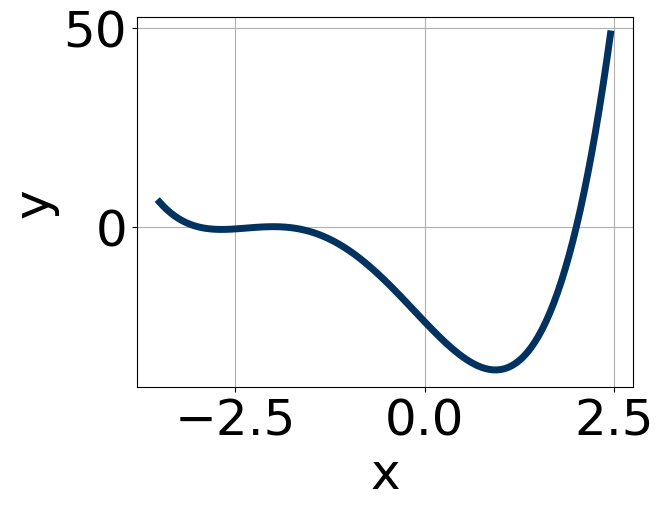
\includegraphics[width=0.5\textwidth]{../Figures/polyGraphToFunctionB.png}
\end{center}
\begin{enumerate}[label=\Alph*.]
\item \( 19(x + 2)^{7} (x - 2)^{4} (x + 3)^{9} \)
\item \( 20(x + 2)^{10} (x - 2)^{8} (x + 3)^{7} \)
\item \( 13(x + 2)^{4} (x - 2)^{11} (x + 3)^{11} \)
\item \( -18(x + 2)^{4} (x - 2)^{7} (x + 3)^{4} \)
\item \( -4(x + 2)^{10} (x - 2)^{11} (x + 3)^{5} \)

\end{enumerate} }
\litem{
Construct the lowest-degree polynomial given the zeros below. Then, choose the intervals that contain the coefficients of the polynomial in the form $ax^3+bx^2+cx+d$.\[ \frac{1}{4}, \frac{7}{5}, \text{ and } 2 \]\begin{enumerate}[label=\Alph*.]
\item \( a \in [17, 26], b \in [68, 75], c \in [69, 74], \text{ and } d \in [10, 16] \)
\item \( a \in [17, 26], b \in [-7, -6], c \in [-59, -56], \text{ and } d \in [-18, -13] \)
\item \( a \in [17, 26], b \in [-73, -66], c \in [69, 74], \text{ and } d \in [-18, -13] \)
\item \( a \in [17, 26], b \in [-73, -66], c \in [69, 74], \text{ and } d \in [10, 16] \)
\item \( a \in [17, 26], b \in [-66, -58], c \in [34, 45], \text{ and } d \in [10, 16] \)

\end{enumerate} }
\litem{
Describe the zero behavior of the zero $x = 2$ of the polynomial below.\[ f(x) = -9(x - 7)^{7}(x + 7)^{4}(x - 2)^{12}(x + 2)^{9} \]\begin{enumerate}[label=\Alph*.]
\begin{multicols}{2}\item 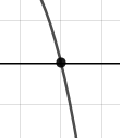
\includegraphics[width = 0.3\textwidth]{../Figures/polyZeroBehaviorCopyAB.png}\item 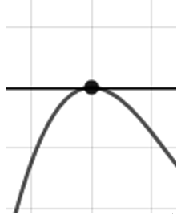
\includegraphics[width = 0.3\textwidth]{../Figures/polyZeroBehaviorCopyBB.png}\item 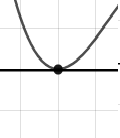
\includegraphics[width = 0.3\textwidth]{../Figures/polyZeroBehaviorCopyCB.png}\item 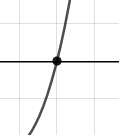
\includegraphics[width = 0.3\textwidth]{../Figures/polyZeroBehaviorCopyDB.png}\end{multicols}\item None of the above.
\end{enumerate} }
\litem{
Describe the end behavior of the polynomial below.\[ f(x) = 8(x - 9)^{2}(x + 9)^{5}(x - 7)^{4}(x + 7)^{6} \]\begin{enumerate}[label=\Alph*.]
\begin{multicols}{2}\item 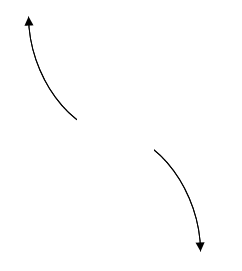
\includegraphics[width = 0.3\textwidth]{../Figures/polyEndBehaviorCopyAB.png}\item 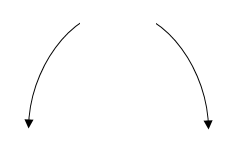
\includegraphics[width = 0.3\textwidth]{../Figures/polyEndBehaviorCopyBB.png}\item 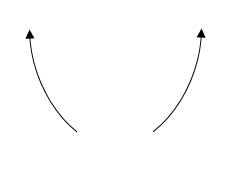
\includegraphics[width = 0.3\textwidth]{../Figures/polyEndBehaviorCopyCB.png}\item 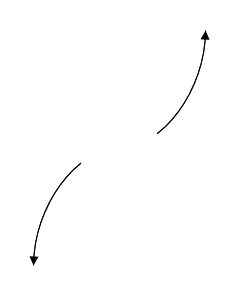
\includegraphics[width = 0.3\textwidth]{../Figures/polyEndBehaviorCopyDB.png}\end{multicols}\item None of the above.
\end{enumerate} }
\litem{
Describe the end behavior of the polynomial below.\[ f(x) = 9(x + 5)^{3}(x - 5)^{6}(x - 3)^{5}(x + 3)^{7} \]\begin{enumerate}[label=\Alph*.]
\begin{multicols}{2}\item 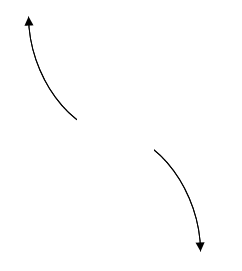
\includegraphics[width = 0.3\textwidth]{../Figures/polyEndBehaviorAB.png}\item 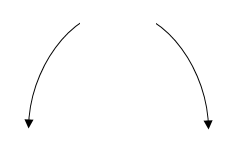
\includegraphics[width = 0.3\textwidth]{../Figures/polyEndBehaviorBB.png}\item 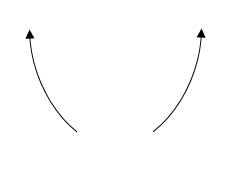
\includegraphics[width = 0.3\textwidth]{../Figures/polyEndBehaviorCB.png}\item 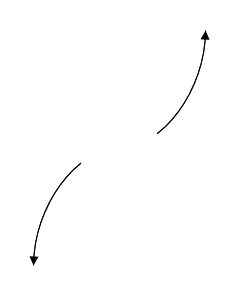
\includegraphics[width = 0.3\textwidth]{../Figures/polyEndBehaviorDB.png}\end{multicols}\item None of the above.
\end{enumerate} }
\litem{
Construct the lowest-degree polynomial given the zeros below. Then, choose the intervals that contain the coefficients of the polynomial in the form $x^3+bx^2+cx+d$.\[ -2 + 5 i \text{ and } 3 \]\begin{enumerate}[label=\Alph*.]
\item \( b \in [-0.1, 2.4], c \in [15, 24], \text{ and } d \in [-94, -80] \)
\item \( b \in [-2.5, -0.9], c \in [15, 24], \text{ and } d \in [75, 89] \)
\item \( b \in [-0.1, 2.4], c \in [-8, -3], \text{ and } d \in [10, 24] \)
\item \( b \in [-0.1, 2.4], c \in [-2, 5], \text{ and } d \in [-10, -2] \)
\item \( \text{None of the above.} \)

\end{enumerate} }
\litem{
Construct the lowest-degree polynomial given the zeros below. Then, choose the intervals that contain the coefficients of the polynomial in the form $ax^3+bx^2+cx+d$.\[ \frac{-3}{2}, \frac{-7}{3}, \text{ and } -4 \]\begin{enumerate}[label=\Alph*.]
\item \( a \in [1, 13], b \in [42, 51], c \in [111, 117], \text{ and } d \in [-87, -83] \)
\item \( a \in [1, 13], b \in [-4, 2], c \in [-76, -68], \text{ and } d \in [84, 88] \)
\item \( a \in [1, 13], b \in [-50, -41], c \in [111, 117], \text{ and } d \in [-87, -83] \)
\item \( a \in [1, 13], b \in [42, 51], c \in [111, 117], \text{ and } d \in [84, 88] \)
\item \( a \in [1, 13], b \in [28, 30], c \in [-3, 5], \text{ and } d \in [-87, -83] \)

\end{enumerate} }
\litem{
Which of the following equations \textit{could} be of the graph presented below?
\begin{center}
    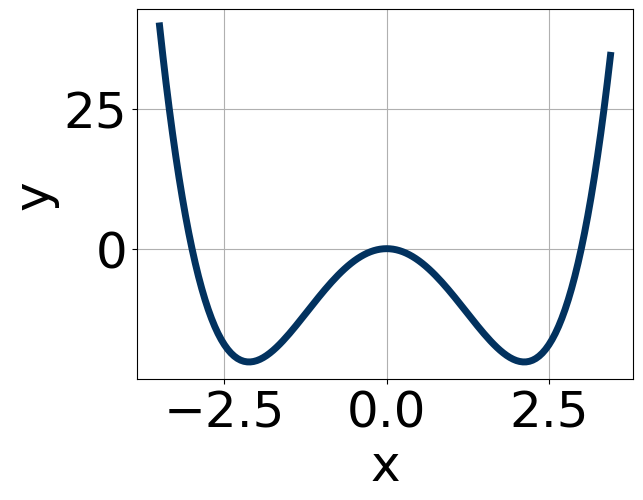
\includegraphics[width=0.5\textwidth]{../Figures/polyGraphToFunctionCopyB.png}
\end{center}
\begin{enumerate}[label=\Alph*.]
\item \( 18x^{8} (x + 3)^{9} (x - 3)^{7} \)
\item \( -19x^{4} (x + 3)^{5} (x - 3)^{4} \)
\item \( 19x^{4} (x + 3)^{8} (x - 3)^{11} \)
\item \( 8x^{5} (x + 3)^{8} (x - 3)^{7} \)
\item \( -3x^{4} (x + 3)^{11} (x - 3)^{7} \)

\end{enumerate} }
\litem{
Construct the lowest-degree polynomial given the zeros below. Then, choose the intervals that contain the coefficients of the polynomial in the form $x^3+bx^2+cx+d$.\[ 5 + 2 i \text{ and } 4 \]\begin{enumerate}[label=\Alph*.]
\item \( b \in [-6, 2], c \in [-9.4, -7.5], \text{ and } d \in [18, 22] \)
\item \( b \in [-21, -8], c \in [67.5, 70.9], \text{ and } d \in [-126, -113] \)
\item \( b \in [-6, 2], c \in [-8, -3.8], \text{ and } d \in [5, 12] \)
\item \( b \in [12, 21], c \in [67.5, 70.9], \text{ and } d \in [115, 119] \)
\item \( \text{None of the above.} \)

\end{enumerate} }
\litem{
Describe the zero behavior of the zero $x = 2$ of the polynomial below.\[ f(x) = 8(x + 2)^{2}(x - 2)^{7}(x - 4)^{9}(x + 4)^{11} \]\begin{enumerate}[label=\Alph*.]
\begin{multicols}{2}\item 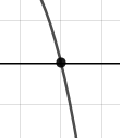
\includegraphics[width = 0.3\textwidth]{../Figures/polyZeroBehaviorAB.png}\item 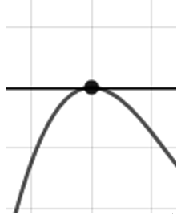
\includegraphics[width = 0.3\textwidth]{../Figures/polyZeroBehaviorBB.png}\item 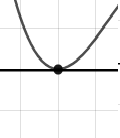
\includegraphics[width = 0.3\textwidth]{../Figures/polyZeroBehaviorCB.png}\item 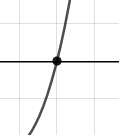
\includegraphics[width = 0.3\textwidth]{../Figures/polyZeroBehaviorDB.png}\end{multicols}\item None of the above.
\end{enumerate} }
\end{enumerate}

\end{document}